\documentclass[11pt,letter]{ivoa}
\input tthdefs

\usepackage[utf8]{inputenc}

\title{Table Access Protocol}

\ivoagroup{Data Access Layer Working Group}

\author{Patrick Dowler, ...}

\editor{Patrick Dowler}

\previousversion[http://www.ivoa.net/Documents/TAP/1.0]{TAP-1.0}
       

\begin{document}

\begin{abstract}
The table access protocol (TAP) defines a service protocol for accessing general 
table data, including astronomical catalogs as well as general database tables. 
Access is provided for both database and table metadata as well as for actual 
table data. This version of the protocol includes support for multiple query 
languages, including queries specified using the Astronomical Data Query 
Language ([std:ADQL]) within an integrated interface. It also includes support 
for both synchronous and asynchronous queries. Special support is provided for
spatially indexed queries using the spatial extensions in ADQL. A multi-position 
query capability permits queries against an arbitrarily large list of 
astronomical targets, providing a simple spatial cross-matching capability. 
More sophisticated distributed cross-matching capabilities are possible by 
orchestrating a distributed query across multiple TAP services.  
\end{abstract}


\section*{Acknowledgments}

The authors would like to acknowledge all contributors to this and previous 
versions of this standard, especially: K. Andrews, J. Good, R. Hanisch, G. 
Lemson, T. McGlynn, K. Noddle, F. Ochsenbein, I. Ortiz, P. Osuna, R. Plante, G. 
Rixon, J. Salgado, A. Stebe, and A. Szalay.


\section*{Conformance-related definitions}

The words ``MUST'', ``SHALL'', ``SHOULD'', ``MAY'', ``RECOMMENDED'', and
``OPTIONAL'' (in upper or lower case) used in this document are to be
interpreted as described in IETF standard, \citet{std:RFC2119}.

The \emph{Virtual Observatory (VO)} is general term for a collection of 
federated resources that can be used to conduct astronomical research, 
education, and outreach. The \href{http://www.ivoa.net}{International
Virtual Observatory Alliance (IVOA)} is a global collaboration of separately 
funded projects to develop standards and infrastructure that enable VO 
applications.


\section{Introduction}
The Table Access Protocol (TAP) is a web-service protocol that gives access to 
collections of tabular data referred to collectively as a tableset.  TAP 
services accept queries posed against the tableset available via the service and 
return the query response as another table, in accord with the relational model. 
 Queries may be submitted using various query languages and may execute 
synchronously or asynchronously. Support for the Astronomical Data Query 
Language ([std:ADQL]) is mandatory; support for other query languages is supported 
but optional.

The result of a TAP query is another table, normally returned as a VOTable. 
Support for VOTable output is mandatory; all other formats are optional.

The table collections made accessible via TAP are typically stored in relational 
database management systems (RDBMS). A TAP service exposes the database schema 
to client applications so that queries can be posed directly against arbitrary 
data tables available via the service.

Multi-table operations such as joins or cross matches are possible provided the 
tables are all managed by the local TAP service, and provided the service 
supports these capabilities.  Larger scale operations such as a distributed 
cross match are also possible, but require combining the results of multiple TAP 
services.

\subsection{Role within the VO Architecture}

NOTE: not in TAP-1.0

\begin{figure}
\centering

% Get the architecture diagram from the TCG chair
% http://wiki.ivoa.net/twiki/bin/view/IVOA/IvoaTCG
% If they give you a PDF, for now dumb it down to a png by
% convert -antialias -density 72x72 archdiag.pdf archdiag.png
% Oh -- Notes don't need this; you'd have to remove archdiag.png
% from FIGURES in the Makefile, too.

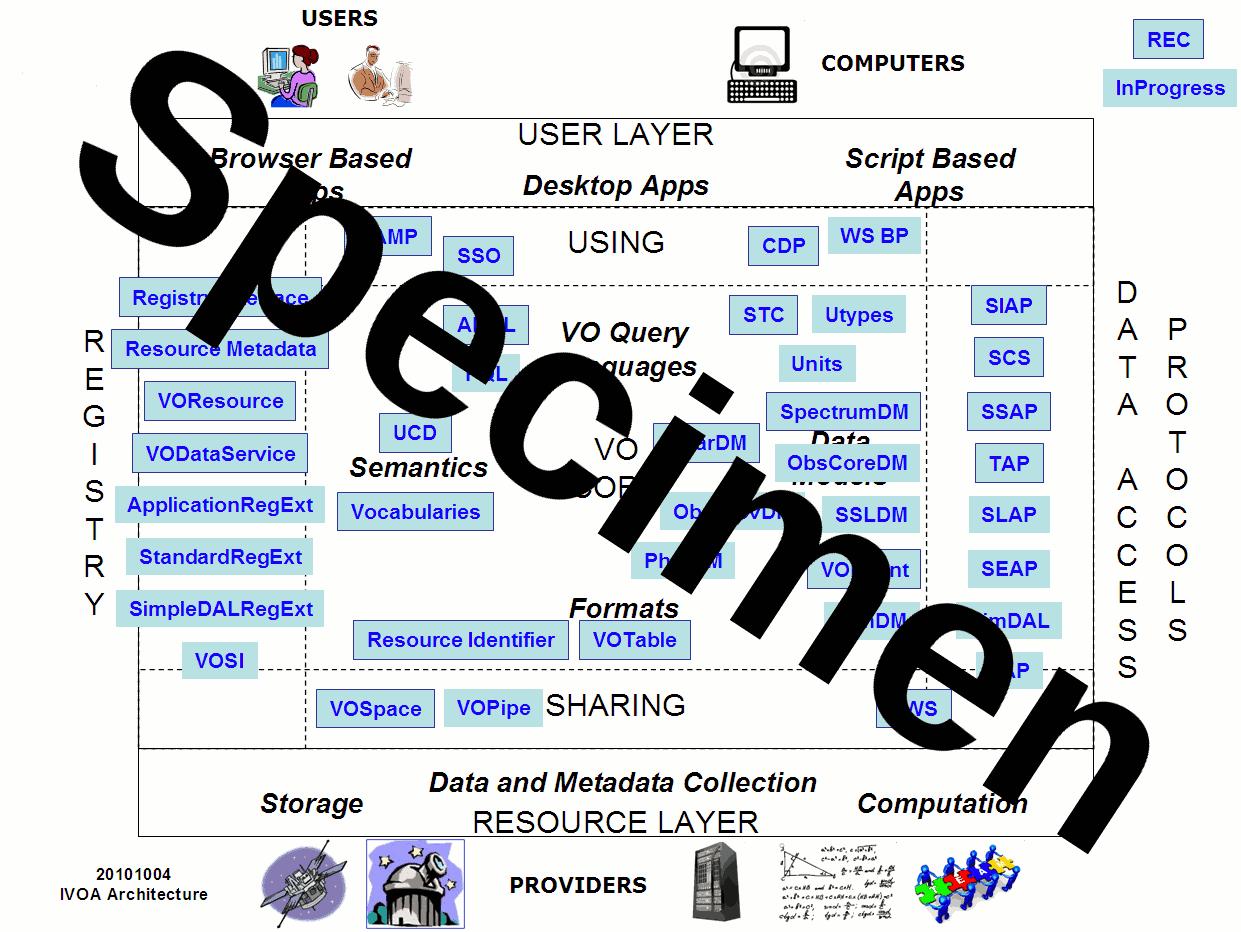
\includegraphics[width=0.9\textwidth]{archdiag.png}
\caption{Architecture diagram for this document}
\label{fig:archdiag}
\end{figure}

Fig.~section~\ref{fig:archdiag} shows the role this document plays within the
IVOA architecture \citep{note:VOARCH}.


\subsection{Motivating Use Cases}
Below are some of the more common use cases that have motivated the development 
of the TAP specification. While this is not complete, it helps to understand the 
problem area covered by this specification.

\subsubsection{Discover Metadata}
Since content in relational databases is often custom and project-specific, 
users of a TAP service must be able to discover the names of tables and 
columns, datatypes, units, and other information necessary to construct 
meaningful correct queries.

\subsubsection{Query Custom Tables}
A large amount of astronomical data and metadata is stored in tables in 
relational databases. Historically, users could query these tables through 
custom user interfaces (usually web page forms), but such approaches could not 
provide support for truly ad-hoc querying. A TAP service should enable users to 
discover and query custom tables with a flexible and expressive input that 
supports ad-hoc querying: selecting output, filtering the result, joining 
multiple tables, computing aggregate quantities, etc. 

\subsubsection{Query Standard Tables}
A TAP service should enable users to query externally defined standard tables 
in a uniform way such that the same web service request can be sent to multiple 
services. Services must be able to declare their support for standard tables in 
the service metadata.

\subsubsection{Query Standard Data Models}
A TAP service should enable users to query (parts of) externally defined data 
models that are (partially or fully) implemented by the service. Services must 
be able to declare their support for data models as well as the way that model 
elements are mapped to tables and columns.

\subsubsection{ADQL Queries}
The Astronomical Data Query Language ([std:ADQL]) is the standard 
query language for the IVOA. Support for ADQL queries is mandatory. ADQL can be 
used to specify queries  that access one or more tables provided by the TAP 
service, including the standard metadata tables. In general, the client must 
access table metadata in order to discover the names of tables and columns and 
then formulate queries. ADQL queries provide a direct (low-level) access to the 
tables; a query will be written for a specific TAP service and will not be 
usable with other services unless the query refers only to common tables and 
columns. It is also possible that the service registration (in an IVOA Registry) 
may include sufficient table metadata to enable queries to be written directly.

\subsubsection{Other Query Languages}
A TAP service must be able to support use of other query languages, such
pass-through of native SQL directly to an underlying DBMS or simple key-vale 
(parameter-based) constraints. The service interface must allow for 
this and the service capabilities must be able to describe it. This mechanism 
also allows future developments within and outside the IVOA to be used without 
revising the TAP specification.

\subsubsection{Asynchronous Queries}
Asynchronous queries allow for long running queries to complete without 
the client maintaining a connection to the service. Results are stored by 
the service for later retrieval by the client. Asynchronous query 
execution is generally more robust and not susceptible to time-outs or other 
transient failures. They are especially suited to queries that run for a long 
time before producing output (e.g. queries that compute or aggregate values).

\subsubsection{Synchronous Queries}
Synchronous queries execute immediately  and the client must wait for the query 
to finish. Synchronous query execution is generally simpler and provides a 
faster (low latency) response and should be adequate when the query will execute 
and start returning results quickly. Even with large query results, synchronous 
queries are a good approach as long as the service can stream the output 
and consume modest internal resources. 


\subsection{Interface Overview -- move to examples section?}
Table Access Protocol (TAP) is implemented over the HTTP protocol using standard 
HTTP GET and POST requests and conventions. A TAP request specifies one or more 
parameter key/value pairs; both keys and values are strings. The keys used are 
discussed in this specification and in the specifications for query languages 
supported by a service. The values may need to be encoded, using standard 
URL-encoding. For the following examples, http://example.com/tap/ is the base 
URL for a TAP service.

This is an example of a synchronous ADQL query on r magnitude:

\begin{verbatim}
HTTP POST htp://example.com/tap/sync
REQUEST=doQuery
LANG=ADQL
QUERY=SELECT * FROM magnitudes as m where m.r>=10 and m.r<=16
\end{verbatim}

Synchronous queries return the table of results in the HTTP response to the 
initial request. In the examples above, the output format defaults to VOTable; 
the FORMAT parameter could be added to select a different format.

Asynchronous queries are created in the same way as the synchronous kind, using 
the /async endpoint:

\begin{verbatim}
HTTP POST http://example.com/tap/async
REQUEST=doQuery
LANG=ADQL
QUERY=SELECT * FROM magnitudes AS m WHERE m.r>=10 AND m.r<=16
\end{verbatim}

The service's response to these requests is a URL representing the query's 
state and progress and where the state may be monitored and controlled. The 
query 
result or an error document can then be retrieved from a URL associated with the 
job. This is an application of the UWS pattern. The query is then executed 
with a separate request to run the job URL:

\begin{verbatim}
HTTP POST http://example.com/tap/async/<jobid>/phase
PHASE=RUN
\end{verbatim}

The state of the job can be retrieved from the phase resource:

\begin{verbatim}
HTTP GET http://example.com/tap/async/<jobid>/phase
\end{verbatim}

The client may have to check the phase multiple times until the job 
finishes. Once the returned value is COMPLETED, the results can be obtained 
from the results resource:

\begin{verbatim}
HTTP GET http://example.com/tap/async/<jobid>/results/result
\end{verbatim}

In addition to the sync and async resources for query execution, a TAP service 
also has metadata resources defined by the VOSI standard. The availability of a 
service can be monitored by accessing:

\begin{verbatim}
HTTP GET http://example.com/tap/availability
\end{verbatim}

The complete table metadata can be obtained:

\begin{verbatim}
HTTP GET http://example.com/tap/tables
\end{verbatim}

The capabilities can be obtained by:

\begin{verbatim}
HTTP GET http://example.com/tap/capabilities
\end{verbatim}

The capabilities are also accessible via a service request to the synchronous 
query resource:

\begin{verbatim}
HTTP GET http://example.com/tap/sync?REQUEST=getCapabilities
\end{verbatim}

This output lists support for optional TAP functionality and additional 
implemented interfaces.

\section{Resources}
\label{sec:resources}

An implementation of a TAP service provides the following RESTful resources 
under the base URL.

\begin{tabular}{l l l l l}
\label{tab:resources}
resource type & resource name & required \\
{sync} & /sync & must (anonymous) & \\
{async} & /async & must (anonymous) & \\
{sync} & service-specific & may (alternate authentication method) & \\
{async} & service-specific & may (alternate authentication method) & \\
VOSI-availability & /availability & should & \\
VOSI-capabilities & /capabilities & must & \\
VOSI-tables & /tables & should & \\
DALI-examples & /examples & should & \\
\end{tabular}

At least one set of {sync} and {async} resources must be named /sync and 
/async respectively for backwards compatibility with TAP-1.0 (which required 
these names. These resources must be used for anonymous query execution. Other 
{sync} and {async} resources may have service specific names, but all resources 
listed above must be siblings so that a client with one such URL can find the 
VOSI-capabilities URL and thus discover other available resources. 

A TAP service must be represented as a set of sibling web resources each 
addressable via a URL in the http scheme, or the https scheme, or both.

The web resource at the root of the tree must represent the service as a whole. 
This specification defines no standard representation for this root resource. 
Implementations may provide a representation, or may return a '404 not found' 
response to requests for the root web-resource. One possible representation is 
an HTML page describing the scientific usage and content of the service. TAP 
clients must not depend on a specific representation of the root web-resource.

\subsection{\{sync\}}
\label{sec:tap-sync}

A TAP service must provide a web resource with relative URL /sync that is a 
direct child of the root web resource. This web resource represents the results 
of synchronous requests. The exact form of the query, and hence the 
representation of the resource, is defined by the  query parameters as listed in 
section~\ref{sec:parameters}. Representations of results of queries if defined in 
section~\ref{sec:RESPONSEFORMAT} and section~\ref{sec:votable}.

For query languages that produce a single result (e.g. ADQL) executed using the 
/sync endpoint, the result of a successful query is returned in the response or 
the response includes an HTTP redirect (303: See Other) to a resource from 
which the result may be retrieved.

An HTTP-GET request to the /sync web resource may return a cached copy of the 
representation. This cached copy might come from an HTTP cache between the 
client and the service, and the service may also maintain its own cache. Clients 
which require an up-to-date representation of volatile data or metadata must use 
HTTP POST.

\subsection{\{async\}}
\label{sec:tap-async}

A TAP service must provide a web resource with relative URL /async that is a 
direct child of the root web resource. This web resource represents controls for 
asynchronous queries. Specifically, the web resource must represent the job-list 
as specified in the UWS standard [std:UWS].

The child web resources of the /async resource are as specified by UWS. These 
are descendants of the /async web-resource, and they include a web resource that 
represents the eventual result of an asynchronous query, e.g.:
\begin{verbatim}
http://example.com/tap/async/42/results/result
\end{verbatim}
where the base URL for the TAP service is:
\begin{verbatim}
http://example.com/tap
\end{verbatim}
the UWS job list is:
\begin{verbatim}
http://example.com/tap/async
\end{verbatim}
and the job resource is
\begin{verbatim}
http://example.com/tap/async/42
\end{verbatim}
where 42 is the job identifier. A client making an asynchronous request must use 
the UWS facilities to monitor or control the job. In addition to the job list 
and job resource above, UWS specifies the name and semantics of the a small set 
of child resources used to view and control the job, e.g.:
\begin{verbatim}
http://example.com/tap/async/42/phase
http://example.com/tap/async/42/quote
http://example.com/tap/async/42/executionduration
http://example.com/tap/async/42/destruction
http://example.com/tap/async/42/error
http://example.com/tap/async/42/parameters
http://example.com/tap/async/42/results
http://example.com/tap/async/42/owner
\end{verbatim}
Successful TAP queries produce results which must be accessible as  resources 
under the UWS result list, e.g.:
\begin{verbatim}
http://example.com/tap/async/42/results/
\end{verbatim}
Failed TAP queries produce an error document (see section~\ref{sec:query-error}) which must be accessible 
as the error resource, e.g.:
\begin{verbatim}
http://example.com/tap/async/42/error
\end{verbatim}
For query languages that produce a single result executed using the /async 
endpoint, the result of a successful query can be found within the result list 
specified by UWS [std:UWS]; the result must be named result and thus clients are able 
to access it directly, e.g.:
\begin{verbatim}
http://example.com/tap/async/42/results/result
\end{verbatim}
Access of this resource must deliver the result, either directly or as an HTTP 
redirect (303: See Other) to a resource from which the result may be retrieved.

For query languages that may produce multiple result resources, the names of the 
results are not specified (they may be specified in the specification for the 
language). The client can always access the result list resource as specified by 
UWS [3].

If the query returned no rows, the result resource must exist and contain no 
data rows. Details on interacting with these resources are specified in the UWS 
standard; for examples specific to TAP see section~\ref{sec:examples} below.

\subsection{/availability}
\label{sec:vosi-availability}

The VOSI availability metadata should be accessible from a web resource with 
relative URL /availability that is a direct child of the root web resource. If 
implemented, the /availability resource must be accessible via the http GET 
method. The content is described by [std:VOSI].

Services which do not implement the /availability resource must respond with an 
HTTP response code of 404 when this resource is accessed.

\subsection{/capabilities}
\label{sec:vosi-capabilities}

The TAP-1.0 standard is identified using 
\begin{verbatim}
ivo://ivoa.net/std/TAP
\end{verbatim}

For TAP-1.1 we define new standard identifiers for each of the 
features. Asynchronous query resources (section~\ref{sec:tap-async}) are described by standardID: 

\begin{verbatim}
ivo://ivoa.net/std/TAP#async-1.1 
\end{verbatim}

Synchronous query resources (section~\ref{sec:tap-sync}) are described by standardID:

\begin{verbatim}
standardID="ivo://ivoa.net/std/TAP#sync-1.1 
\end{verbatim}

In TAP-1.0 the base URL was described with a single standard identifier; in 
TAP-1.1 and beyond, individual resources are described with their on 
standardID. This allows service providers to describe multiple resources that 
deliver the specified feature (e.g. with different authentication methods) in 
the VOSI-capabilities resource.

The VOSI standard specifies that the capability metadata is encoded as an XML 
document which lists each of the service's capabilities as a <capability> 
element. The type of this element (which defines the contents) is 
{http://www.ivoa.net/xml/VOResource/v1.0}Capability from the VOResource XML 
standard [8].

In addition, the capabilities output must also comply with the following    
requirements:

* the returned document must include <capability> elements 
that describes the service's support for the TAP protocol using the TAP and 
VOSI standardID values

* this capability element must include at least one <interface> element 
with its "role" attribute set to "std",  

Note: VO registries recognize a service's support for a standard protocol 
through this capability description. In particular, a different standard 
Capability sub-type is used for each standard protocol to provide capability 
metadata that is specific to that protocol. At the time of this writing, a 
Capability sub-type for TAP has not yet been defined. Thus for compliance with 
this standard, any legal Capability description that meets the above 
restrictions is sufficient. However, once a VOResource extension for TAP is 
standardized, it is strongly recommended that TAP services emit its 
capabilities using that the Capability sub-type specialized for TAP.

For example, the returned capabilities document for a service supporting  TAP 
might look as follows:

\begin{verbatim}
<?xml version="1.0" encoding="UTF-8"?>

<vosi:capabilities xmlns=""
   xmlns:vosi="http://www.ivoa.net/xml/VOSI/v1.0"
   xmlns:vs="http://www.ivoa.net/xml/VODataService/v1.0"
   xmlns:xsi="http://www.w3.org/2001/XMLSchema-instance"
   xsi:schemaLocation="http://www.ivoa.net/xml/VOSI/v1.0
                       http://www.ivoa.net/xml/VOSI/v1.0
             http://www.ivoa.net/xml/VODataService/v1.0
             http://www.ivoa.net/xml/VODataService/v1.0">

  <vosi:capability standardID="ivo://ivoa.net/std/TAP#async-1.1">
    <interface xsi:type="vs:ParamHTTP" role="std">
      <accessURL use="base"> http://myarchive.net/myTAP/async </accessURL>
    </interface>
  </vosi:capability>

  <vosi:capability standardID="ivo://ivoa.net/std/TAP#sync-1.1">
    <interface xsi:type="vs:ParamHTTP" role="std">
      <accessURL use="base"> http://myarchive.net/myTAP/sync </accessURL>
    </interface>
  </vosi:capability>

  <vosi:capability standardID="ivo://ivoa.net/std/VOSI#capabilities">
    <interface xsi:type="vs:ParamHTTP">
      <accessURL use="full">
        http://myarchive.net/myTAP/capabilities </accessURL>
    </interface>
  </vosi:capability>

  <vosi:capability standardID="ivo://ivoa.net/std/VOSI#availability">
    <interface xsi:type="vs:ParamHTTP">
      <accessURL use="full">
        http://myarchive.net/myTAP/availability
      </accessURL>
    </interface>
  </vosi:capability>

  <vosi:capability standardID="ivo://ivoa.net/std/VOSI#tables">
    <interface xsi:type="vs:ParamHTTP">
      <accessURL use="full">
        http://myarchive.net/myTAP/tables </accessURL>
    </interface>
  </vosi:capability>

</vosi:capabilities>
\end{verbatim}

The service capabilities must be accessible from a web resource with relative 
URL /capabilities that is a direct child of the root web resource. The 
/capabilities resource must be accessible via the http GET method. The content 
is described by [8].

\subsection{/tables}
\label{sec:vosi-tables}

The table metadata should be accessible from a web resource with relative URL 
/tables that is a direct child of the root web resource. The /tables resource 
must be accessible via the http GET method. The content is described by 
[std:VODataService] and is equivalent to the metadata from the 
TAP\_SCHEMA described in section~\ref{sec:tap-schema}.

Services which do not implement the /tables resource must respond with an HTTP 
response code of 404 when this resource is accessed.

\subsection{/examples}
\label{sec:dali-examples}

A GET from this endpoint MUST yield a document with a MIME type of either 
application/xhtml+xml or text/html. A service that does not provide examples 
MUST return a 404 HTTP status on accessing this resource.

If present, the endpoint must be represented in a capability in the TAP 
service's registry record. The capability's standardID is defined by 
[std:DALI]. A capability element could hence look like this:

\begin{verbatim}
   <capability standardID="ivo://ivoa.net/std/DALI#examples">
     <interface xsi:type="vr:WebBrowser">
       <accessURL use="full">http://myarchive.net/myTAP/examples</accessURL>
     </interface>
   </capability>
\end{verbatim}

TAP defines two additional properties for the examples vocabulary:

* query -- each example MUST have a unique child element with simple text 
content having a property attribute valued query. It contains the query itself, 
preferably with extra whitespace for easy human consumption and editing. This 
will usually be a HTML pre element.
    
* table -- examples MAY also have descendants with property attributes having 
the value table. These must have pure text content and contain fully qualified 
table names to which the query is somehow "pertaining". Suitable HTML elements 
holding these include span, or a (which would allow linking to further 
information on the table).

When using elements with src or href attributes to carry the property 
attributes, note that the element content must be repeated in a content 
attribute, as otherwise RDFa clients would interpret the embedded link rather 
than the element content as the object in the triple.

TODO: add example(s) here

\subsection{Parameters}
\label{sec:parameters}

The \{async\} and \{sync\} web-resources must accept the parameters listed in 
the following sub-sections. In a synchronous request, the parameters select the 
representation returned in the response message. In an asynchronous request, the 
parameters select the representation of the eventual query result rather than 
the response to the initial request.

Requirements on the presence and values of parameters described below are 
enforced only when the TAP request is executed (not when individual HTTP 
requests are handled). Thus, for asynchronous TAP queries, the parameter 
requirements must be satisfied (and errors returned if not) only when the query 
is run in (in the sense of UWS job execution). Specifically, asynchronous 
queries may be created with with no parameters and multiple, subsequent HTTP 
POST actions may specify the parameters in any order.

Not all combinations of the parameters are meaningful. For example, if a request 
carries  LANG=ADQL then the SELECT parameter (from PQL) is spurious. If a 
service receives a spurious parameter in an otherwise correct request, then the 
service must ignore the spurious parameter, must respond to the request normally 
and must not report errors concerning the spurious parameter.

\subsubsection{REQUEST - remove? }
This parameter distinguishes current service operations, makes it possible to 
extend the service specification (with additional or custom operations), and 
specifies how other parameters should be interpreted. If a TAP service attempts 
to execute a TAP request without this parameter or with an incorrect value for 
this parameter, then the service must reject the request and return an error 
document as the result.

These are the standard values of the parameter:

doQuery: execute a query 

getCapabilities: return VOSI-capabilities metadata 

All requests to execute a query using a query language must 
include REQUEST=doQuery and must include the LANG parameter. For other values of 
REQUEST, additional parameters may or may not be required. The 
REQUEST=getCapabilities service operation must be supported for synchronous 
(/sync) requests and is not defined for asynchronous (/async) requests.

For synchronous queries, the HTTP request must also include additional 
parameters (see below) with the details of the query. These are used for 
metadata queries and data queries.

For asynchronous queries, the additional parameters may be included with the 
HTTP request that creates the query (the UWS job) or they may be POSTed directly 
to the created job resource, in one or more separate HTTP requests. The 
parameter names remain the same in both cases.

\subsubsection{LANG}
\label{sec:LANG}

The LANG parameter specifies the query language. The service must support LANG 
and the client must provide a value with REQUEST=doQuery. The only standard 
values for the LANG parameter is ADQL (a required language). Support for other 
languages and the LANG value to use with them is described in the service 
capabilities.

For example, an ADQL query would be performed with
\begin{verbatim}
REQUEST=doQuery
LANG=ADQL
QUERY=<ADQL query string>
\end{verbatim}
A PQL query would be performed with
\begin{verbatim}
REQUEST=doQuery
LANG=PQL
<PQL-specific parameters>
\end{verbatim}
The value of LANG is a string specifying the language and optionally the 
language version used for the query parameter(s), as defined by the service 
capabilities.  The client may specify the version of the query language,  e.g. 
LANG=ADQL-2.0 (the syntax should be as shown) or it may omit the version, e.g. 
LANG=ADQL.  The service should return an “unknown query language” error as 
described in section~\ref{sec:query-error} if an unsupported language or an incompatible 
language version is specified.

\subsubsection{QUERY}
\label{sec:QUERY}

The QUERY parameter is used to specify the ADQL query. It may also be used to 
specify the query for other values of LANG (e.g. LANG=<some RDBMS-specific SQL 
variant>) which are not specified in this document but may be described in the 
service capabilities.

A service must support the QUERY parameter because ADQL is a required language.  
The case sensitivity of the query string is defined solely by the query language 
specification. In the case of ADQL 2.0, for example, the query is not case 
sensitive except for character  literals; schema, table, and column names, 
function names, and other ADQL keywords are not case sensitive.

Within the ADQL query, the service must support the use of timestamp values as 
described in [std:DALI].

If the tables that are queried through a service contain columns with spatial 
coordinates and the service supports spatial querying via the ADQL “region” 
constructs, the service must support the INTERSECTS function and it must support 
the following geometry functions: REGION, POINT, BOX, CIRCLE, COORD1, COORD2, 
COORDSYS. Support for the AREA, CONTAINS, and POLYGON functions are optional. If 
the service supports the REGION function, it must support region encoding in 
STC-S format (see section 6 ); the extent of STC-S support within the REGION 
function is left up to the implementation. Coordinate system specification for 
POINT, BOX, CIRCLE, and POLYGON must use values from STC-S as described in ???.

Note: Although it is allowed by the ADQL syntax, clients should be careful when 
mixing constants and column references for coordinate system and coordinate 
values. For example, POINT('ICRS', t.ra, t.dec) does not cause t.ra and t.dec to 
be transformed to ICRS; it simply tells the service to treat the values  as 
being expressed in that coordinate system.

\subsubsection{FORMAT and RESPONSEFORMAT}
\label{sec:RESPONSEFORMAT}

The RESPONSEFORMAT parameter is fully described in [std:DALI]. For backwards 
compatibility, TAP-1.1 must also accept the FORMAT parameter as equivalent to 
RESPONSEFORMAT.

\subsubsection{MAXREC}
\label{sec:MAXREC}

The MAXREC parameter and its effect on the query result is fully described in 
[std:DALI]. If the result set is truncated in this fashion, it must include an 
overflow indicator as specified in section XREF.

For the special value of MAXREC=0, the service is not required to execute the 
query; a successful  MAXREC=0 request does not necessarily mean that the query 
is valid and the overflow indicator does not necessarily mean that there is at 
least one row satisfying the query. The service may perform validation and may 
try to execute the query, in which case a MAXREC=0 request can fail. A query 
with MAXREC=0 can be used with a simple query (e.g. SELECT * FROM  
some\_table) to extract and examine the VOTable metadata (assuming 
FORMAT=votable). Note: in this version of TAP, this is the only mechanism to 
learn some of the detailed metadata, such as coordinate systems used.

\subsubsection{RUNID}
The RUNID parameter is fully described in [std:DALI].

\subsubsection{VERSION}
The VERSION parameter is fully described in {std:DALI].

\subsubsection{UPLOAD}
\label{sec:UPLOAD}

The UPLOAD parameter is described in [std:DALI]. Services should support the 
upload of temporary tables (in [std:VOTable] format) via the standard UPLOAD 
parameter. The table-name(s) must be legal ADQL table names as defined in 
[std:ADQL] but restricted as described below XREF. URIs maybe be simple URLs 
(e.g. with a URI scheme of http) or URIs (e.g. with a URI scheme of vos or 
param) that must be resolved to give the location of the table content. See 
section XREF for details.

If table upload supported, the service must accept tables in VOTable format. 
The client specifies the name of the uploaded table; this name must be a legal 
ADQL table name with no catalog or schema (i.e., a string following the 
regular identifier production of [std:ADQL]). Uploaded tables must be referred 
to in queries as TAP\_UPLOAD.<tablename>, where <tablename> is the 
specified by the user. Tables in the TAP\_UPLOAD schema are 
transient and persist only for the lifetime of the query (although caching might 
be used behind the scenes) and are never visible in the 
TAP\_SCHEMA metadata.

The [std:DALI] UPLOAD parameter supports both external resources and in-line 
content. For external resources, one provides a URI (usually an HTTP URL) the 
TAP service can use to obtain the table content. For example,
\begin{verbatim}
HTTP POST http://example.com/tap/async/42
UPLOAD=mytable,http://otherplace.com/path/votable.xml
\end{verbatim}
The service would retrieve the table from the provided URL and 
make it visible to the query as TAP\_UPLOAD.mytable.

If the TAP service supports VOSpace (TBD: how to declare this?), one may 
specify an upload table using a URI to a table stored in a VOSpace, for example:
\begin{verbatim}
HTTP POST http://example.com/tap/async/42
UPLOAD=mytable,vos://space/path/votable.xml
\end{verbatim}
The service would resolve the URI, contact the VOSpace, retrieve the table, and 
make it visible to the query as TAP\_UPLOAD.mytable.

UPLOADs are accumulating, i.e., each UPLOAD parameter given will create one or 
more tables in TAP\_UPLOAD. When the table names from two or more 
upload items agree after case folding, the service behaviour is unspecified. 
Clients thus cannot reliably overwrite uploaded tables; to correct errors, they 
have to tear down the existing job and create a new one. In principle, any 
number of tables can be uploaded using the UPLOAD parameter and any combination 
of URI schemes supported by the service as long as they are assigned unique 
table names within the query. Services may limit the size and number of 
uploaded tables; if the service refuses to accept the entire table it must 
respond with an error as described in section~\ref{sec:query-error}.


\section{Use of VOTable}
\label{sec:votable}

The [std:VOTable] format is the standard format for output (query results) and 
input (table upload) in a TAP service. 


\subsection{INFO elements}
\label{sec:vot-info}

The RESOURCE element must contain an INFO element with attribute 
name="QUERY\_STATUS" indicating the success of the operation. For 
RESOURCE elements that contain a TABLE element, this INFO element must appear 
lexically before the TABLE. The following values are defined for this INFO 
element's value attribute:

“OK”, meaning that the query executed successfully and a result table is 
included in the resource 

"ERROR”, meaning that an error was detected at the level of the TAP 
protocol or the query failed to execute 

The content of the INFO element conveying the status should be a message 
suitable for display to the user describing the status.

\begin{verbatim}
<INFO name="QUERY_STATUS" value="OK"/>
\end{verbatim}
 
\begin{verbatim}
<INFO name="QUERY_STATUS" value="OK">Successful query</INFO>
\end{verbatim}

\begin{verbatim}
<INFO name="QUERY_STATUS" value="ERROR">
   value out of range in POS=45,91
</INFO>
\end{verbatim}

Additional INFO elements may be provided, e.g., to echo the input parameters 
back to the client in the query response (a useful feature for debugging or to 
self-document the query response), but clients should not depend on these. 

\begin{verbatim}
<RESOURCE type=”results”>
<INFO name="QUERY_STATUS" value="ERROR">
    unrecognized operation
</INFO>
<INFO name="SPECIFICATION" value="TAP"/>
<INFO name=”VERSION” value=”1.0”/>
<INFO name="REQUEST" value="doQuery"/>
<INFO name="baseUrl" value="http://webtest.aoc.nrao.edu/ivoa-dal"/>
<INFO name="serviceVersion" value="1.0"/
...
</RESOURCE>
\end{verbatim}

If an overflow occurs (result exceeds MAXREC), the service must close the table 
and append another INFO element to the RESOURCE (after the TABLE) with 
name=”QUERY\_STATUS” and the value=”OVERFLOW”.
\begin{verbatim}
<RESOURCE type=”results”>
<INFO name="QUERY_STATUS" value="OK"/>
...
<TABLE>...</TABLE>
<INFO name="QUERY_STATUS" value="OVERFLOW"/>
</RESOURCE>
\end{verbatim}

In the above example, the TABLE should have exactly MAXREC rows.

If an error occurs while writing the rows of the VOTable, the service must 
close the table and append another INFO element to the RESOURCE, after the 
TABLE, with name=”QUERY\_STATUS” and the value=”ERROR”.
\begin{verbatim}
<RESOURCE type=”results”>
<INFO name="QUERY_STATUS" value="OK"/>
...
<TABLE>...</TABLE>
<INFO name="QUERY_STATUS" value="ERROR" />
</RESOURCE>
\end{verbatim}
The content of these trailing INFO elements is optional and intended for users; 
client software should not depend on it.

Thus, one INFO element with name=”QUERY\_STATUS” and value=”OK” or 
value=”ERROR” must be included before the TABLE. If the TABLE does not contain 
the entire query result, one INFO element with value=”OVERFLOW” or 
value=”ERROR” must be included after the table. 

\subsection{Successful Queries}
\label{sec:query-ok}

The result of a query depends on the query language used and may be one or more 
tables in one or more resources. Unsupportable combinations of query result and 
FORMAT (e.g. queries that produce multiple tables and an inherently 
single-table format like CSV) will cause the request to fail. Currently, an ADQL 
query result must be a single table (in a single file).

The output table must include the same number and order of columns as specified 
in the SELECT clause of the query. For VOTable output, the name attribute of 
FIELD elements must be the same as the column names (or aliases if specified in 
the query) from the query and the datatype, arraysize, and xtype attributes of 
FIELD elements must be set using the mapping specified in section 2.5 . The 
xtype attribute in the output must match the datatype for the column in the 
TAP\_SCHEMA.

VOTable structure follows the rules in section 2.9 and must be returned with an 
allowed VOTable MIME type (application/x-votable+xml or text/xml). If the 
RESPONSEFORMAT parameter (section~\ref{sec:RESPONSEFORMAT}) of the request 
specified a specific VOTable MIME type, the requested MIME type must be used 
in the HTTP response.

CSV formatted data should represent the output table with one row of text per 
table row, with the table column values rendered as text and separated by 
commas. If a column value contains a comma the entire column value should be 
enclosed in double quotes.  Text lines may be arbitrarily long.  The first data 
row should give the column name as the data value.   CSV data must be returned 
with a MIME type of text/csv; if the optional header line (with column names) 
is included, the MIME type must be text/csv;header=present. Full details of CSV 
format are defined in RFC 4180 [std:CSV].

TSV formatted data should represent the output table with one row of text per 
table row, with the table column values rendered as text and separated by the 
TAB character. TSV data must be returned with a MIME type of 
text/tab-separated-values [std:TSV]. Column values may not contain the TAB 
character.

\subsection{Errors}
\label{sec:query-error}

If the service detects an exceptional condition, it must return an error 
document with an appropriate HTTP-status code. TAP distinguishes three classes 
of exceptions.

Errors in the use of the HTTP protocol. 

Errors in the use of the TAP protocol, including both invalid requests and 
failure of the service to complete valid requests. 

Error documents for HTTP-level errors are not specified in the TAP protocol. 
Responses to these errors are typically generated by service containers and 
cannot be controlled by TAP implementations. There are several cases where a 
TAP 
service could return an HTTP error. First, the /async endpoint could return a 
404 (not found) error if the client accesses a job within the UWS joblist that 
does not exist. Second, access to a resource could result in an HTTP 401 (not 
authorized) error if authentication is required or an HTTP 403 (forbidden) 
error if the client is not allowed to access the resource.

Error documents for TAP errors must be VOTable documents;  any result-format 
specified in the request is ignored. If the error document is being retrieved 
from the /async/<jobid>/error resource (specified by UWS) after an asynchronous 
query, the HTTP status code should be 200. If the error document is being 
returned directly after a synchronous query, the service may use an appropriate 
HTTP status code, including 200 (successfully returning a response to the 
request) and various 4xx and 5xx values. The exception condition must be 
described to the client using a status code in the VOTable header.  Section   
2.9 specifies the use of VOTable for error documents in TAP services. 

\subsection{Overflows}
\label{sec:query-overflow}

If a query is executed by a TAP service, the number of rows in the table of 
results may exceed a limit requested by the user (using the MAXREC parameter) 
or a limit set by the service implementation (the default or maximum value of 
MAXREC). In these cases, the query is said to have 'overflowed'. Typically, a 
TAP service will not detect an overflow until some part of the table of results 
has been sent to the client.

If an overflow occurs, the TAP service must produce a table of results that is 
valid, in the required output format, and which contains all the results up to 
the point of overflow. Since an output overflow is not an error condition, the 
MIME type of the output must be the same as for any successful query and the 
HTTP status-code must be as for a successful, complete query.

If the output format is VOTable, section 2.9.1 describes the method by which 
the overflow is reported. No method of reporting an overflow is defined for 
formats other than VOTable.

\subsection{VOTable vs RDBMS Tables and Columns}
\label{sec:votable-rdbms}

TODO: describe the bi-directional mapping of VOTable <-> RDBMS table aka the 
old section on uploading tables... should this come earlier in the doc?

The column names in the transient database table are taken directly from the 
name attribute of the VOTable FIELD and PARAM elements. TODO: add column name 
restrictions here to avoid quoted identifiers. The datatypes of the 
transient table are determined from the FIELD and PARAM attributes as follows:

TODO: something like the table from TAP-1.0

The default mapping of data types are shown above (no arraysize or xtype). If 
the xtype attribute is set, this is the preferred internal datatype. If xtype is 
not set, then the datatype and arraysize indicate the most suitable internal 
datatype. Note that the last column of Table (x) is not normative. 
Implementations SHOULD try to make sure that the actual types chosen are at 
least signature-compatible with the recommended types (i.e., integers should 
remain integers, floating-point values floating-point values, etc.), such that 
clients can reliably write queries against uploaded tables.

For columns with xtype adql:REGION, this is particularly critical, since 
databases typically use different types to represent various STC-S objects. 
Clients are advised to assume that such columns will be approximated with 
polygons in the actual database table.

In the arraysize column above, [1] means the arraysize is not set or is set to 
1, n means arraysize is set to a specific value, * means arraysize=”*”, and n* 
means arraysize=”n*” (variable size up to length n). A blank means the arraysize 
is not set.

Binary values (unsignedByte in VOTable, BINARY, VARBINARY, or BLOB in ADQL) can 
be expressed as specified by the VOTable standard. By default, VOTable allows 
them to be written as an array of decimal numbers, e.g. 12 56 0 255 0 0 255 (one 
number per byte value).

For columns of type BLOB or CLOB, most database systems support reference to 
these columns in the select clause but not in any other part of the query. 
Services may use these types to indicate that columns may only be selected. For 
example, if service implementors want to make URL(s) available as column values 
in the results, but do not actually store the URL(s) in the database, they would 
specify a column with xtype=”adql:CLOB” and the column with URL(s) could be 
referenced in the SELECT clause of a query, but could not be used in the WHERE 
clause. The service could then process the query result and insert the URL(s) 
or, more likely, transform a column value (an identifier) into a URL while 
writing the results.

TIMESTAMP values are specified as described in [std:DALI]. The 
xtype=”adql:TIMESTAMP” attribute must be specified in an uploaded VOTable in 
order for the values to be inserted in a column of type TIMESTAMP; without the 
xtype, the values would be inserted into a CHAR(n) or VARCHAR column.

POINT and REGION values are specified in STC-S format (see section 6 ). The 
xtype=”adql:POINT” attribute must be specified in an uploaded VOTable in order 
for the char values to be parsed and treated as POINTs (e.g. to be used with 
some of the ADQL region functions). For regions, the xtype=”adql:REGION” 
attribute must be specified in an uploaded VOTable in order for the char values 
to be parsed and treated as REGIONs (e.g. to be used with some of the ADQL 
region functions).

\section{Metadata: TAP\_SCHEMA}
\label{sec:tap-schema}

There are several approaches to getting metadata for a given TAP service. All 
TAP services must support a set of tables in a schema named 
TAP\_SCHEMA that describe the tables and columns included in the 
service. In addition to the TAP\_SCHEMA, there are two other ways 
to get metadata from a TAP service. First, the VOSI tables resource provides 
metadata on all tables and columns; this resource is described in 2.2.5 . The 
VOSI tables resource provides the same metadata as the TAP\_SCHEMA 
but in a rigorously controlled format; the information in the 
TAP\_SCHEMA is equivalent to that defined by the  VODataService 
[7]. Second, the client may specify a query of one or more tables setting the 
MAXREC parameter to 0 so that only the metadata regarding the requested fields 
is returned. Use of MAXREC is described in section~\ref{sec:MAXREC}.

The TAP\_SCHEMA provides access to table, column, and join key 
metadata through the TAP query mechanisms themselves. Users can discover tables 
or columns that meet their specific criteria by querying the tables described 
below.  The service may enhance the TAP\_SCHEMA with additional 
metadata where that seems appropriate; since it is self-describing, the 
TAP\_SCHEMA may be queried to determine if any extended schema 
metadata is defined by the service. Services must provide these tables and make 
them accessible by all supported query mechanisms.

The qualified names in the tables of the TAP schema must follow the rules 
defined in section 2.4. The names must be stated in a form that is acceptable as 
an operand of a query.

All columns in the TAP\_SCHEMA tables are of type VARCHAR except 
for size,  principal, indexed, and std (in Columns) which are INTEGER values.

Implementors are permitted to include additional tables in the 
TAP\_SCHEMA to describe additional aspects of their service not 
covered by this specification. Implementors may also include additional columns 
in the standard tables described below. For example, one could include a column 
with a timestamp saying when metadata values were was last modified.

\subsection{Schemas}
\label{sec:tap-schema-schemas}

The table TAP\_SCHEMA.schemas must contain the following columns:

\begin{tabular}{l l l}
\label{tab:resources}
column name & datatype & not-null \\
schema\_name & VARCHAR & true \\
utype & VARCHAR & false \\
description & VARCHAR & false \\
\end{tabular}

The schema\_name values must be unique and may be qualified by the 
catalog name or not depending on the implementation requirements. The fully 
qualified schema name is defined by the ADQL language and  follows the pattern 
[catalog.]schema. The schema metadata are included for reference and are not 
used directly to construct queries.

\subsection{Tables}
\label{sec:tap-schema-tables}
The table TAP\_SCHEMA.tables must contain the following columns:

\begin{tabular}{l l l}
\label{tab:tap-schema-tables}
column name & datatype & not-null \\
schema\_name & VARCHAR & true \\
table\_name & VARCHAR & true \\
table\_type & VARCHAR & true \\
utype & VARCHAR & false \\
description & VARCHAR & false \\
\end{tabular}

The table\_name values must be unique. The value of the 
table\_name should be the string that is recommended for use in 
querying the table; it may or may not be qualified by schema and catalog name(s) 
depending on the implementation requirements. The fully qualified table name is 
defined by the ADQL language and follows the pattern [[catalog.]schema.]table. 

\subsection{Columns}
\label{sec:tap-schema-columns}
The table TAP\_SCHEMA.columns must contain the following columns:

\begin{tabular}{l l l}
\label{tab:tap-schema-columns}
column name & datatype & not-null \\
table\_name & VARCHAR & true \\
column\_name & VARCHAR & true \\
datatype & VARCHAR & true \\
"size" arraysize? datasize? & INTEGER & false \\
description & VARCHAR & false \\
utype & VARCHAR & false \\
unit & VARCHAR & false \\
ucd & VARCHAR & false \\
indexed & BOOLEAN? & true \\
principal & BOOLEAN? & true \\
std & BOOLEAN? & true \\
\end{tabular}

The table\_name,column\_name (pair) values must be 
unique.

Data types and how they map to VOTable datatypes are described in Section 
xref{sec:vot-rdbms} above. The “size” gives the length of variable length datatypes, 
for example varchar(256); this size does not map to the VOTable arraysize attribute 
when the latter specifies the size and shape of a multi-dimensional array. To use the 
size column in a query, it must be put in double quotes since it collides with an ADQL reserved 
word. Since delimited identifiers are case-sensitive, for the size column both 
clients and servers MUST always (in particular, in the DDL for 
TAP\_SCHEMA) use lower case exclusively. In the next major version 
of TAP, this column will be called arraysize.

The “principal” flag indicates that the column is considered a core part the 
content; clients can use this hint to make the principal column(s) visible, for 
example by selecting them by default in generating an ADQL query. In cases where 
the services selects the columns to return (such as PQL without a SELECT 
parameter), the principal column indicates those columns that are returned by 
default. 

The “indexed” flag indicates that the column is indexed, potentially 
making queries run much faster if this column is used in a constraint. 

The “std” is included for compatibility with the registry, which uses this value 
to indicate that a given column is defined by some standard, as opposed to a 
custom column defined by a particular service.

\subsection{Foreign Keys}
\label{sec:tap-schema-keys}
The table TAP\_SCHEMA.keys must contain the following columns to 
describe foreign key relations between tables:

\begin{tabular}{l l l}
\label{tab:tap-schema-keys}
column name & datatype & not-null \\
key\_id & VARCHAR & true \\
from\_table & VARCHAR & true \\
target\_table & VARCHAR & true \\
description & VARCHAR & false \\
utype & VARCHAR & false \\
\end{tabular}

The key\_id values are unique and used only to join with the 
TAP\_SCHEMA.key\_columns table below. There may be 
one or more rows with different key\_id values and a pair 
of tables to denote one or more ways to join the tables.

The table TAP\_SCHEMA.key\_columns must contain the 
following columns to describe the columns that make up a foreign key:

\begin{tabular}{l l l}
\label{tab:tap-schema-key-columns}
column name & datatype & not-null \\
key\_id & VARCHAR & true \\
from\_column & VARCHAR & true \\
target\_column & VARCHAR & true \\
\end{tabular}

There may be one or more rows with a specific key\_id to 
denote single or multi-column keys.

A TAP service must provide the tables listed above and may provide other tables 
in the TAP\_SCHEMA namespace.


\section{Examples}
\label{sec:examples}

The UWS pattern is specified in [std:UWS] and its application to TAP in section 
section~\ref{sec:tap-async}. This section gives examples of the exchange of messages between a 
TAP client and service when using UWS to run an asynchronous query.

\subsection{Example: Asynchronous Query}
Consider a TAP service at http://example.com/tap. TAP mandates that the 
asynchronous requests be directed to http://example.com/tap/async (e.g. for 
anonymous queries). This URL points to the list of 'jobs'; i.e. the list of 
queries currently or recently executed.

\subsubsection{Creating a Query}
To create a new query, the client POSTs a request to the job list:

\begin{verbatim}
HTTP POST http://example.com/tap/async
REQUEST=doQuery
LANG=ADQL
QUERY=SELECT TOP 100 * FROM foo
\end{verbatim}

The service then creates a job and assigns that job a name and a URL based on 
the name. Suppose that the name is 42, then the URL will be 
http://example.com/tap/async/42 because the jobs are always children of the job 
list. While the job is in the PENDING phase, additional parameters may be 
specified by additional POSTs to the job resource, for example:

\begin{verbatim}
HTTP POST http://example.com/tap/async/42
UPLOAD=mytable,http://a.b.c/mytable.xml
\end{verbatim}

After each such POST, the service issues an HTTP redirection to the job's URL, 
where the modified state may be accessed:

\begin{verbatim}
HTTP status 303 'See other'
Location: http://example.com/tap/async/42
\end{verbatim}

All TAP-specific parameters are stored using the paramList mechanism of UWS and 
are included in the XML representation of the job:
\begin{verbatim}
HTTP GET http://example.com/tap/async/42
\end{verbatim}
or directly from the parameters resource:
\begin{verbatim}
HTTP GET http://example.com/tap /async/42/parameters
\end{verbatim}
Individual parameters cannot be accessed as separate web resources.

The UWS pattern requires the following resources to describe and control the 
job:
\begin{verbatim}
http://example.com/tap/async/42/phase
http://example.com/tap/async/42/quote
http://example.com/tap/async/42/executionduration
http://example.com/tap/async/42/destruction
http://example.com/tap/async/42/results
http://example.com/tap/async/42/error
\end{verbatim}
The quote resource specifies the predicted completion time for the job (query), 
assuming it is started immediately. In practice, it is very hard to estimate the 
time a query will take; for TAP services it is recommended that this be set to 
the current time plus the maximum amount of time the query will be allowed to 
run (see termination below). 

The termination resource specifies the amount of time (in seconds) the job 
(query) will be allowed to run before being aborted by the service. The 
termination time is set by the service and can be read from the job or directly 
from the termination resource:

\begin{verbatim}
HTTP GET http://example.com/tap/async/42/executionduration
\end{verbatim}
The service may allow the client to change the termination:
\begin{verbatim}
HTTP POST http://example.com/tap/async/42/executionduration
TERMINATION=600
\end{verbatim}
The destruction resource specifies when the service will destroy the job. The 
service is only required to keep a job for a finite period of time, after which 
it may destroy the job, including the result. After this time, the client will 
receive an HTTP 404 'not found' status if it tries to get any information about 
the job. The destruction time of the job is chosen by the service and the client 
can read it from the job or directly from the destruction resource:
\begin{verbatim}
HTTP GET http://example.com/tap/async/42/destruction
\end{verbatim}
The service may allow the client to change the destruction time:
\begin{verbatim}
HTTP POST http://example.com/tap/async/42/destruction
DESTRUCTION=2008-11-11T11:11:11Z
\end{verbatim}

\subsubsection{Running a Query}
The phase URL shows the progress of the job. When the job is created by the 
service it will normally be set to PENDING, but might be set to ERROR if the 
service has rejected the job. If the phase is ERROR, then the error URL should 
lead to a an error document explaining the problem. If the phase is PENDING, 
then the client needs to commit the job for execution.

The client runs the job by posting to the phase URL:
\begin{verbatim}
HTTP POST http://example.com/tap /async/42/phase
PHASE=RUN
\end{verbatim}

The service replies with a redirection to the job URL
\begin{verbatim}
HTTP status 303 'see other'
Location: http://example.com/tap /async/42
\end{verbatim}
The phase will now have changed to either QUEUED or EXECUTING, depending on the 
service implementation. The client tracks the execution by polling the phase 
URL:
\begin{verbatim}
HTTP GET http://example.com/tap/async/42/phase
\end{verbatim}
A job in the  QUEUED or EXECUTING phase may be aborted by posting to the phase 
URL:
\begin{verbatim}
HTTP POST http://example.com/tap/async/42/phase
PHASE=ABORT
\end{verbatim}

When the query is complete, the phase changes to COMPLETED. The client then 
retrieves the result from the results list:
\begin{verbatim}
HTTP GET http://example.com/tap/async/42/results/result
\end{verbatim}
The client knows that the table of results is at the URL /result relative to the 
results list because the TAP protocol requires this naming. A generic UWS client 
could find the name of the result and retrieve it by examining either the job 
description:
\begin{verbatim}
HTTP GET http://example.com/tap/async/42
\end{verbatim}
or by looking specifically at the result list:
\begin{verbatim}
HTTP GET http://example.com/tap/async/42/results
\end{verbatim}
If the service cannot run the query, then the final phase is ERROR and there is 
no table of results. In this case, the client should expect an HTTP 404 'not 
found' status if it tries to retrieve the result. The client should look instead 
at the error resource to find out what went wrong:
\begin{verbatim}
HTTP GET http://example.com/tap/async/42/error
\end{verbatim}
If the job was aborted (by the client or the service), the final phase will be 
ABORTED and there is no table or results. As with errors, the client should look 
at the error resource to find out what went wrong.

The basic sequence can be executed from a web browser or from a shell script 
using the curl utility:
\begin{verbatim}
curl -d 'REQUEST=doQuery&LANG=PQL&POS=12,34&SIZE=0.5&FROM=foo' \
       http://example.com/tap/async

  [read Location header from curl output]

curl -d 'PHASE=RUN' http://example.com/tap/async/42

curl http://example.com/tap/async/42/phase

  [repeat until phase is COMPLETED]

curl http://example.com/tap/42/results/result
\end{verbatim}

\subsubsection{Example: Synchronous Query}

TODO

\subsubsection{Example: DALI-examples Document}

TODO

\section{Use of STC-S in TAP - deprecated}

NOTE: The old section 6 is not included from TAP-1.0 since it was informative 
and does not belong in this document. If we need to define syntax for 
points, circles, and polygons then that should be done in [std:DALI], which 
already defines timestamp syntax. 

\section{VOSpace Integration - deprecated}

Note: some text moved to the UPLOAD section; may propose DEST parameter for 
outout.

\section{Use of HTTP - deprecated}
Note: This section is in or belongs in DALI.

\appendix

\section{Changes from Previous Versions}

\subsection{Changes from TAP-1.0}

Restructured the document and removed text that duplicates material from DALI. 
Rewrite the overly long introduction with some basic use cases to help define 
the scope and tell readers what TAP is supposed to accomplish.

Made clarifications: restricted allowed table names for UPLOAD, clarified that 
multiple UPLOAD pamaters accumulate, deprecated the size column in 
TAP\_SCHEMA.columns and added advice to quote it as a delimited 
identifier, made presence of a TABLE element on VOTable output only required for 
successful queries, added optional DALI-examples endpoint (text TBD).

Defined standardID values for the async and sync resource types and explicitly 
allow for multiple of each resource (typically to support authentication). The 
fixed paths /async and /sync are still required and are to provide anonymous 
query access, which should be compatible with existing services.

\bibliography{ivoatex/ivoabib}


\end{document}
